% ------------------------------------------------------------------------------
% TYPO3 Version 9.3 - What's New - Chapter "Backend User Interface" (English Version)
%
% @author	Michael Schams <schams.net>
% @license	Creative Commons BY-NC-SA 3.0
% @link		http://typo3.org/download/release-notes/whats-new/
% @language	English
% ------------------------------------------------------------------------------
% LTXE-CHAPTER-UID:		07b25346-95b1df21-a6ebe09a-49f53f41
% LTXE-CHAPTER-NAME:	Backend User Interface
% ------------------------------------------------------------------------------

\section{Interfaccia utente Backend}
\begin{frame}[fragile]
	\frametitle{Interfaccia utente Backend}

	\begin{center}\huge{Capitolo 1:}\end{center}
	\begin{center}\huge{\color{typo3darkgrey}\textbf{Interfaccia utente Backend}}\end{center}

\end{frame}

% ------------------------------------------------------------------------------
% LTXE-SLIDE-START
% LTXE-SLIDE-UID:		95e3703a-3fa83dbe-818c08a9-ebcc6b12
% LTXE-SLIDE-TITLE:		Search Engine Optimization
% ------------------------------------------------------------------------------

\begin{frame}[fragile]
	\frametitle{Interfaccia utente Backend}
	\framesubtitle{Search Engine Optimization}

	Le proprietà di pagina hanno un nuovo tab "SEO", che permette agli utenti di BE di configurare
	le informazioni relative al SEO, dati \href{http://ogp.me/}{Open Graph} e molto altro.

	\begin{figure}
		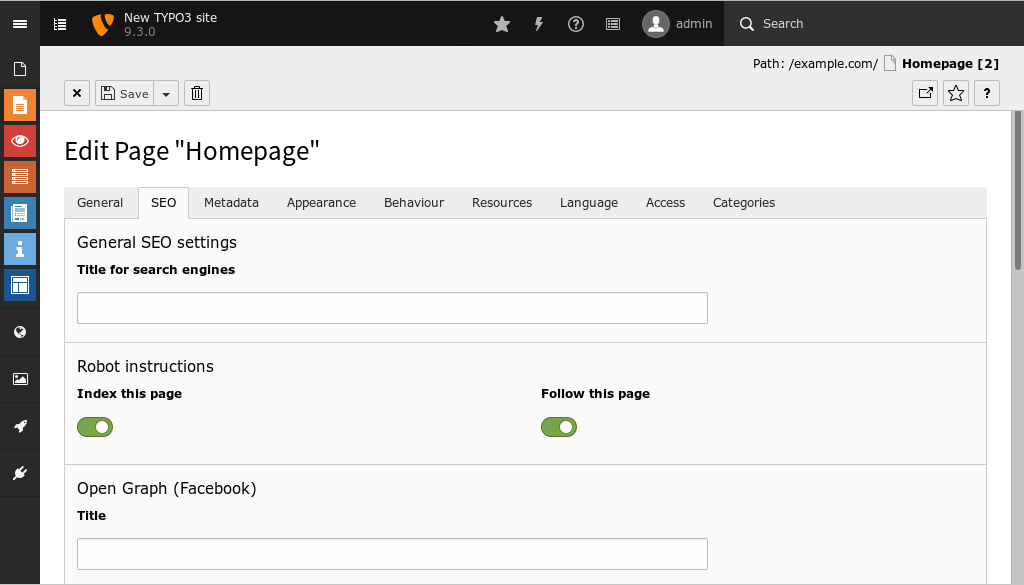
\includegraphics[width=0.70\linewidth]{BackendUserInterface/SearchEngineOptimizationPageProperties.png}
	\end{figure}

\end{frame}

% ------------------------------------------------------------------------------
% LTXE-SLIDE-START
% LTXE-SLIDE-UID:		db23afdf-d3e51a96-848b71c9-51bb6a64
% LTXE-SLIDE-TITLE:		Filebrowser Search (Image Meta Data)
% LTXE-SLIDE-REFERENCE:	#71644 - Add metadata to filebrowser search
% ------------------------------------------------------------------------------

\begin{frame}[fragile]
	\frametitle{Interfaccia utente Backend}
	\framesubtitle{Ricerca Filebrowser}

	Quando si usa la funzionalità di ricerca in \textbf{FILE → Filelist}, i meta data
	dei file (es. campo "Titolo", "Descrizione" e "Testo alternativo") sono anch'essi usati per
	la ricerca.

	\begin{figure}
		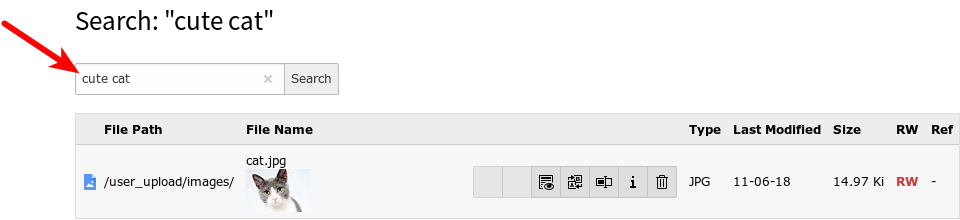
\includegraphics[width=0.90\linewidth]{BackendUserInterface/FilebrowserSearchMetaData.png}
	\end{figure}

\end{frame}

% ------------------------------------------------------------------------------
